\documentclass{article}
\usepackage{CJKutf8, indentfirst, graphicx, subfigure}
\begin{document}
\begin{CJK}{UTF8}{bsmi}
\title{硬體設計與實驗 Lab1 Report}
\author{
104021219 鄭余玄
}
\date{}
\maketitle
\section{實做過程}
lab1-1、lab1-2 和 lab1-3 基本上大同小異,只差是在描述的方式不同。
雖然之前數位邏輯設計沒有教過 ALU,但是看完老師作業的敘述之後,很快就能夠上手了。
我是先從 behavioral 的描述開始完成,接者再一路拆解到更細的結構,
這樣即使是在寫 gate level 的描述,也不會被一堆線弄的頭昏眼花。

因為 lab1-4 aluctr 的 01、10、11 訊號都是 bitwise 運算,
所以 4-bit ALU 其實就只是逐位元送到 1-bit ALU 而已。
至於 00 訊號,在仔細思考後,就會發現原理就如同 ripple carry adder,
而訊號 e 就等同於 carry-in,接到下一個訊號 c 的輸入就行了。

\subsection{Block diagram}
\begin{figure*}[h]
\centering{
\hfill
  \subfigure[]{ \label{fig:sub1}
  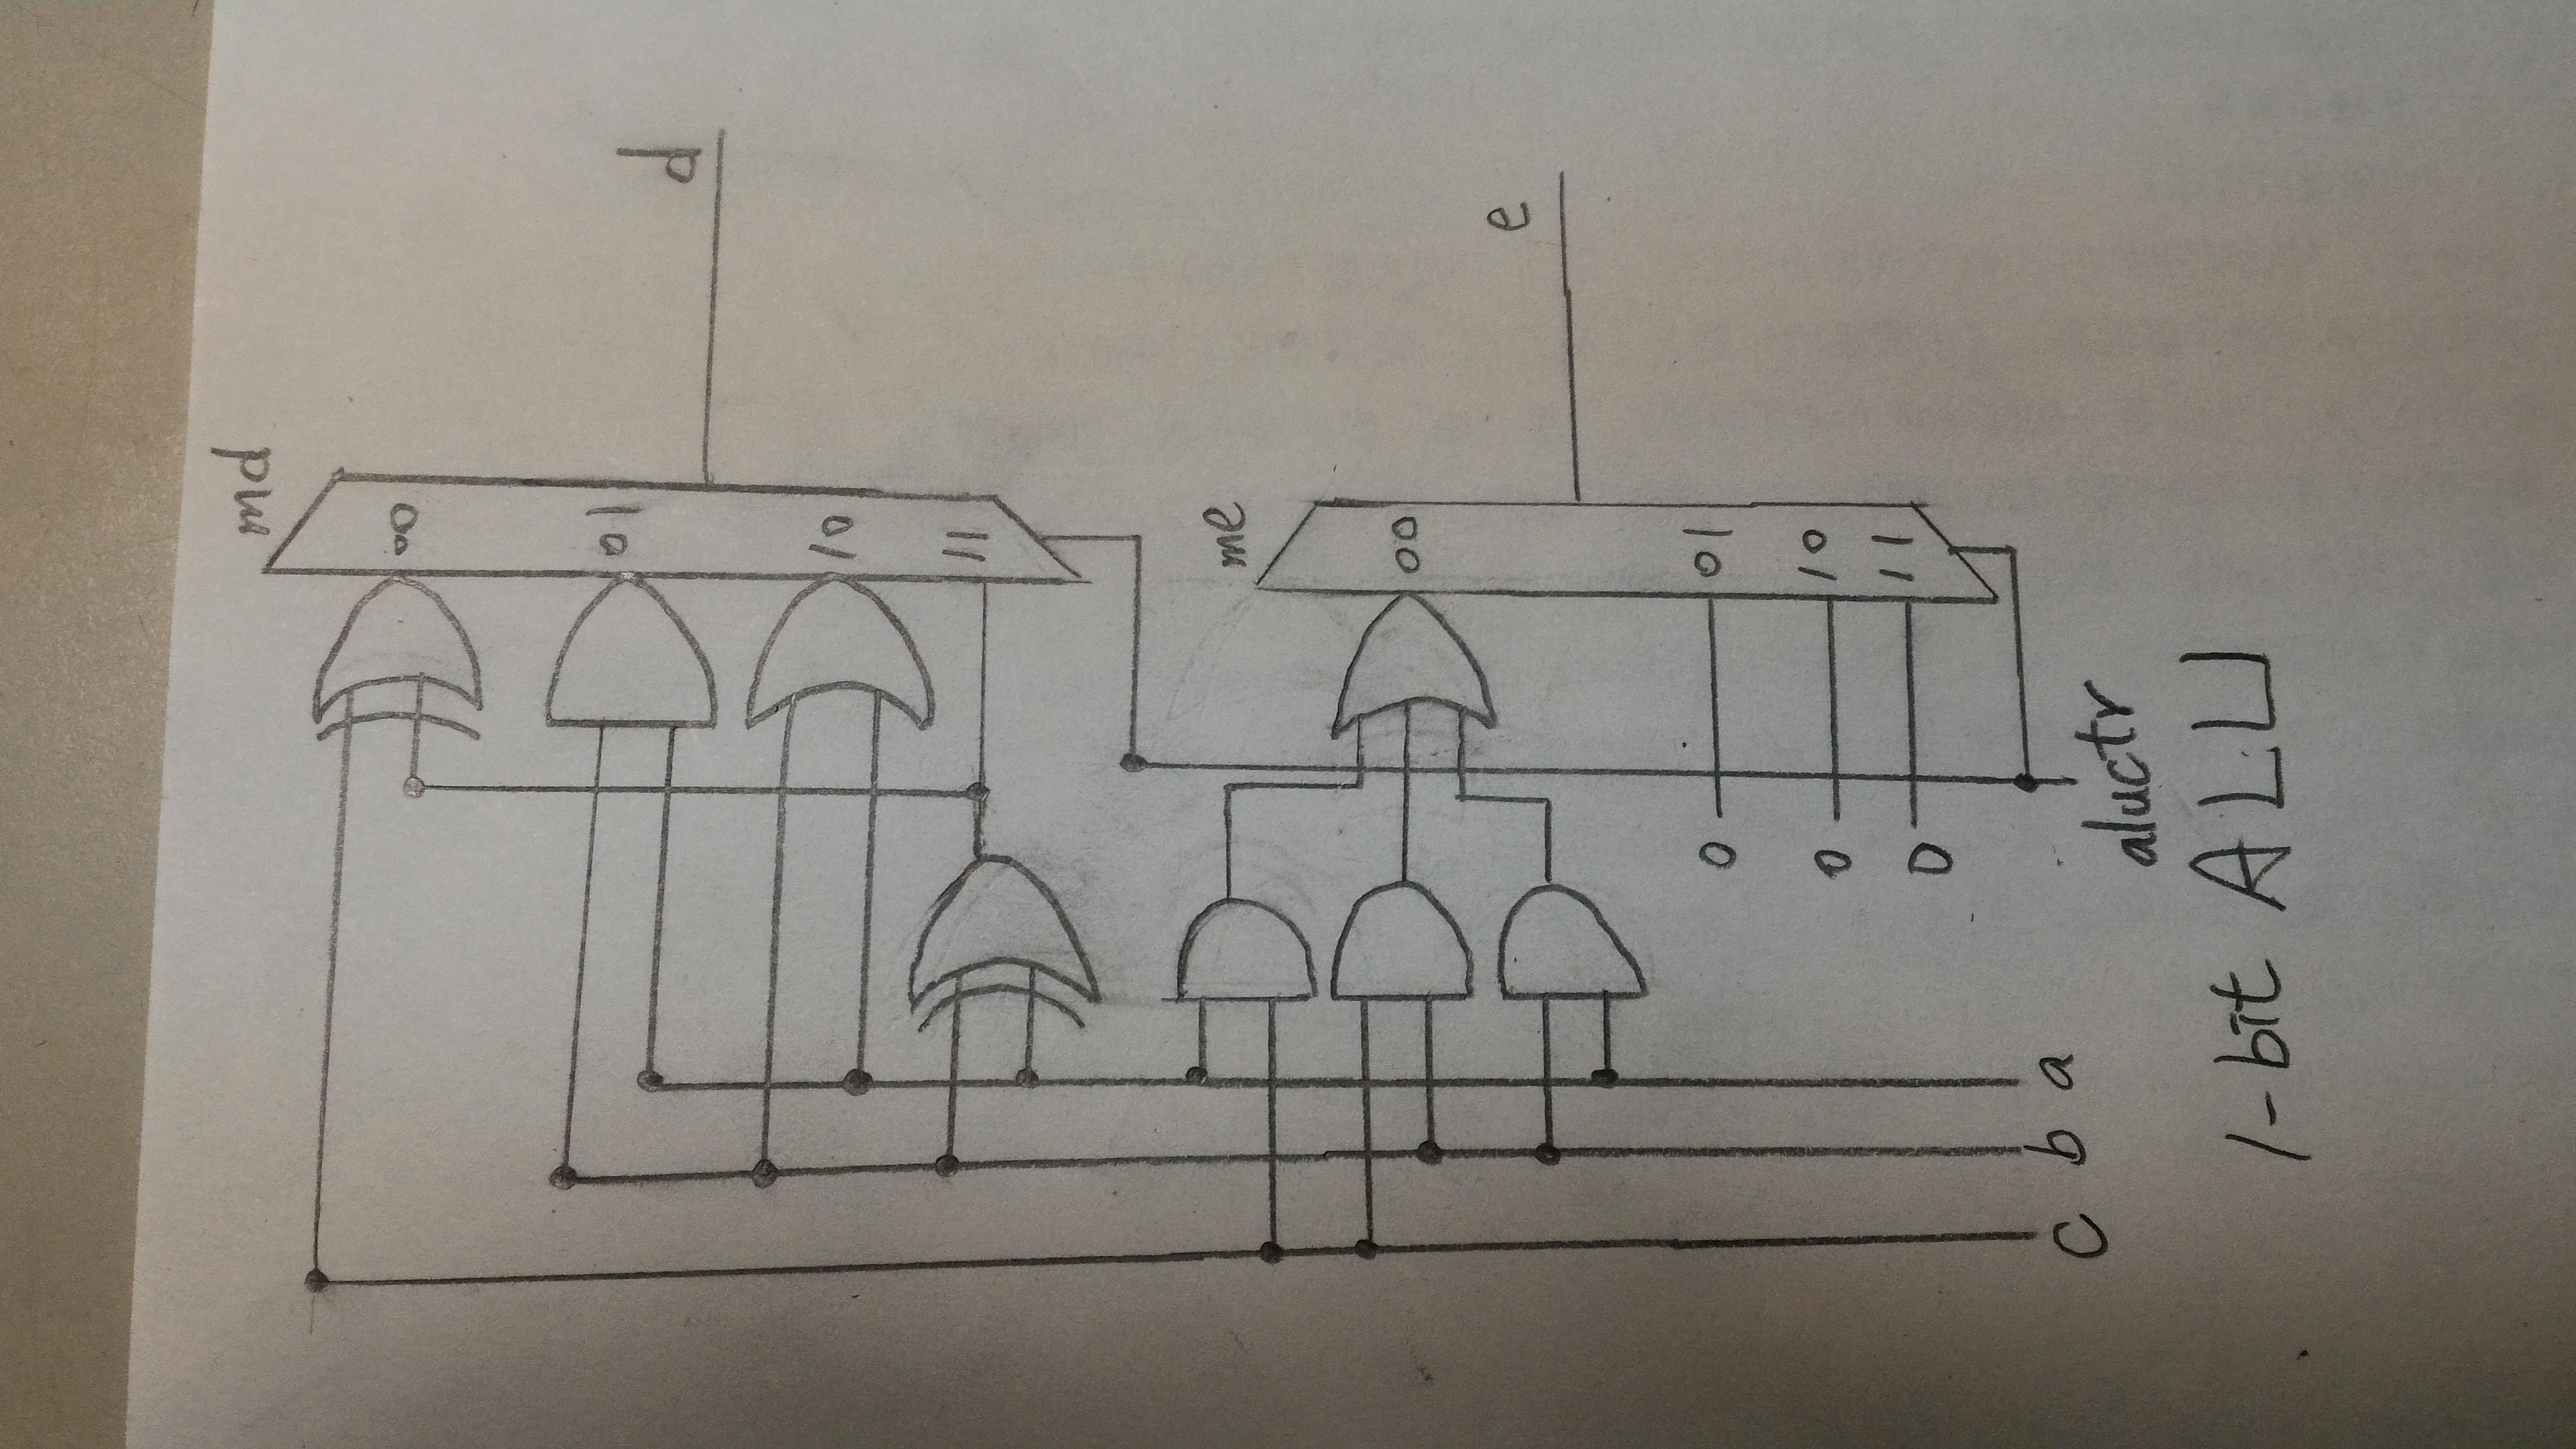
\includegraphics[width=.8\textwidth, angle=270]{1-bit-ALU}
}
\hfill
  \subfigure[]{ \label{fig:sub2}
    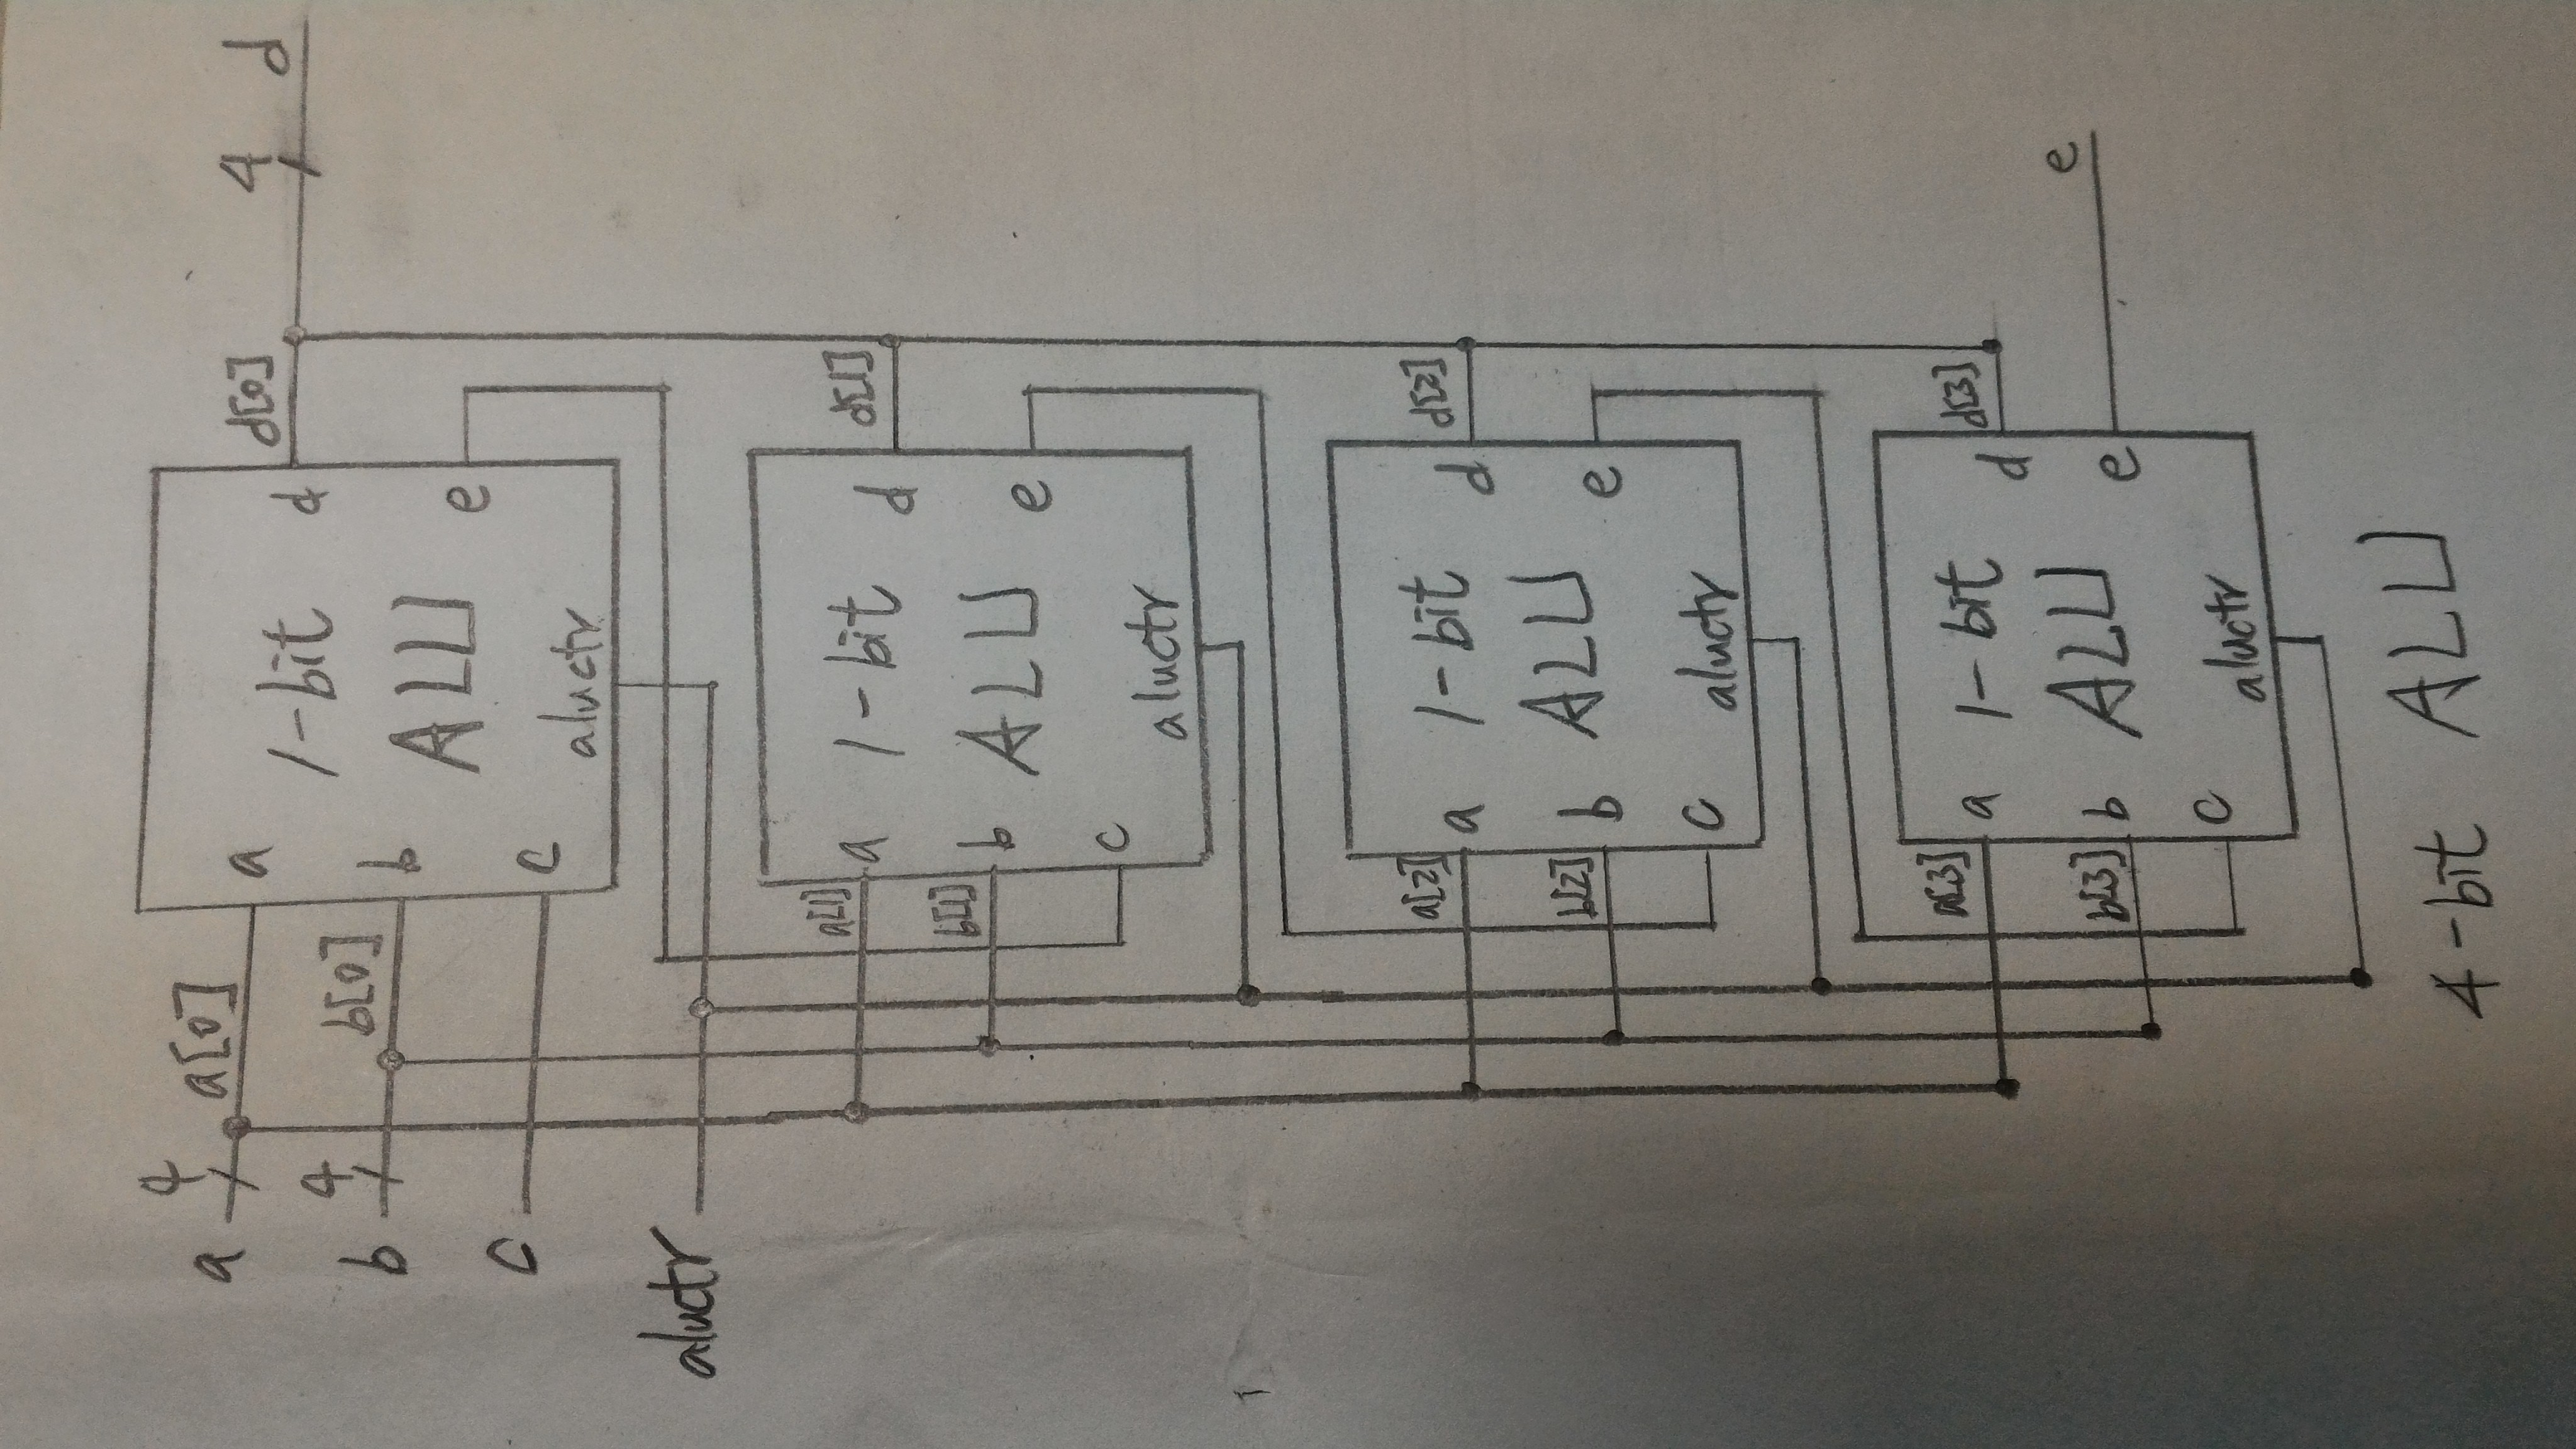
\includegraphics[width=.8\textwidth, angle=270]{4-bit-ALU}
  }
\hfill
}
\caption{Block diagrams: (a) 1-bit ALU and (b) 4-bit ALU.}
\end{figure*}
基本上 gate level 的描述就是圖 \ref{fig:sub1},而 mux 是利用助教所提供的檔案。
\section{心得}
這次實驗花最多時間主要是在安裝、設定和摸索 vivado。
一開始因為程式安裝在 /opt/Xilinx/ 目錄下需要 root 權限,所以直接執行會一直跳 error。
除了權限問題以外,x64 架構的電腦還需要執行一些 shell script 等等諸如此類有點瑣碎的設定。
在經歷種種的障礙排除以後,才有辦法開始寫這次實驗的作業。

此外,這次在跑 simulation 的時候,一開始忘了把 module 改成要測試的,因此在我故意要測試錯誤的情況時,仍然只會輸出 lab1\_1 的 PASS 訊息。這次實驗整體而言,除了安裝 vivado 以外,都算是十分順利,希望以後每次實驗也能如此。
\end{CJK}
\end{document}